\section{Convolutional Neural Networks} \label{sec:cnn}
Convolutional Neural Networks (CNN) are a particular type of Artificial Neural Network (ANN). Similarly to ANNs, it receives an input and returns an output, through a series of hidden layers. Furthermore, it learns its weights and biases by minimising an error function, and performing backpropagation. 

In contrast to ANNs, where each input is fully connected with neurons of the next layer, CNN instead has sparse connectivity. In fact, each neuron in the hidden layer is connected only to a local part of the input. In high-dimensional scenario full connectivity would be wasteful and the extremely large number of parameters would rapidly lead to overfitting. Moreover, CNN make the assumption that the inputs are images, constraining the architecture of the layers in 3 dimensions: \textit{width}, \textit{height}, \textit{depth}. An intuition of the structure is given below:

\begin{figure}[htbp]
	\centering
	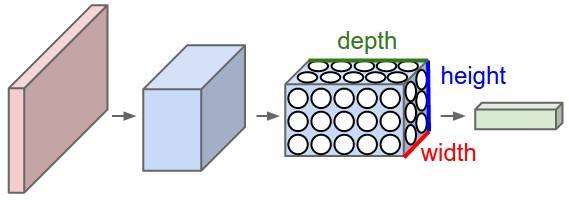
\includegraphics[scale=0.5]{cnn.png}
	\caption{The architecture of a CNN, where each layer is organised in three dimensions. Notice that each layer transforms a 3D input to a 3D output. Graphic sourced from \cite{CS231n}}
	\label{CNN}
\end{figure}
\vspace{0.3cm}
A CNN is represented as a list of layers, where each layer transforms an input volume to an output volume through a differentiable function. There are distinct type of layers and activation functions; a typical structure could contain:
\begin{itemize}
	\item \textbf{Input:} layer holds the input image, for example a [128x128x3] volume for an image of width 128, height 128 and 3 channels for the colors RGB. 
	\item \textbf{Convolution:} layer computing output of neurons that are connected to a local regions of the input. This is done by performing dot products between region connected and weights. As a result we obtain another volume, for example of size [128x128x12]. The depth parameter is analogous of the number of hidden layers in ANN, and it controls the number of neuron in the Convolution layer that connect the same local region of the input volume. 
	%\item \textbf{Relu:} function that perform elementwise activation of the component of the volume, for example \textit{max}(0, $x$). Notice that in this stage the dimension of the volume is unchanged. 
	\item \textbf{Max Pooling:} layer that reduces the dimension of the image (width and height), by selecting the maximum entry of a given region. For example, it takes the maximum of a [2x2] window along the spatial dimensions.
	\item \textbf{Fully connected:} layer that correspond to the final classification of CNN. If there are 10 classes, it will be a [1x1x10] volume containing the score for each category. Fully connected layer have full connections to all activations in the previous layer, as in ANN. 
\end{itemize}

In this way, a CNN converts the original input image to the final category score, layer by layer. In the same way of ANN, the parameters of the network will be trained with gradient descent.

Building an efficient CNN involves a correct tuning of different parameters. Firstly, the \textit{depth} of convolution layers has to be chosen; it will control the number of neurons that connect to the same region of the input volume. Secondly, we need to fix the \textit{receptive field}, which is the size of the local region of the input that we will convolve. Thirdly, we have to specify the \textit{stride} with which the receptive field will look at the input image; the bigger the stride, the smaller the output volume. Finally, sometimes it is necessary to pad the input volume with zeros along the borders; so we need also to specify this parameter, called \textit{padding} that allow us to control the spatial size of the output volume. 

